\documentclass[journal]{IEEEtran}
\usepackage[pdftex]{graphicx}
\usepackage{epstopdf}
\usepackage{cite}


\ifCLASSINFOpdf
   \usepackage[pdftex]{graphicx}
  % declare the path(s) where your graphic files are
   \graphicspath{{../pdf/}{../jpeg/}}
  % and their extensions so you won't have to specify these with
  % every instance of \includegraphics
\DeclareGraphicsExtensions{.pdf,.jpeg,.png}
\else

\fi

\usepackage{amsmath} % assumes amsmath package installed
\usepackage{amssymb}  % assumes amsmath package installed
\DeclareMathOperator*{\argmin}{argmin}

\interdisplaylinepenalty=2500
\usepackage{array}

\usepackage{threeparttable}
\hyphenation{op-tical net-works semi-conduc-tor}


\begin{document}
%
% paper title
% can use linebreaks \\ within to get better formatting as desired
% Do not put math or special symbols in the title.
%\title{Classification of Massive Electrocardiogram Signals with Autoencoder-Based Deep Neural Network}
\title{Deep Learning-Based Classification of Massive Electrocardiography Data}
%
%
% author names and IEEE memberships
% note positions of commas and nonbreaking spaces ( ~ ) LaTeX will not break
% a structure at a ~ so this keeps an author's name from being broken across
% two lines.
% use \thanks{} to gain access to the first footnote area
% a separate \thanks must be used for each paragraph as LaTeX2e's \thanks
% was not built to handle multiple paragraphs
%

\author{Yan~Yan,~
        Xingbin~Qin,~
        Jianping~Fan,~
        and~Lei~Wang~% <-this % stops a space
\thanks{Y. Yan is with the Shenzhen Key Laboratory for Low-cost Healthcare, Shenzhen Institutes of Advanced Technology, Chinese Academy of Sciences. No. 1068, Xueyuan Road, Nanshan District,
Shenzhen, Guangdong Province, China-mail: (yan.yan@siat.ac.cn).}% <-this % stops a space
\thanks{X. Qin is with the Shenzhen Institutes of Advanced Technology, Chinese Academy of Sciences.
No. 1068, Xueyuan Road, Nanshan District, Shenzhen, Guangdong Province, China.}% <-this % stops a space
\thanks{J. Fan is with the Shenzhen Institutes of Advanced Technology, Chinese Academy of Sciences. No. 1068, Xueyuan Road, Nanshan District, Shenzhen, Guangdong Province, China.}% <-this % stops a space
\thanks{L. Wang is with the Shenzhen Key Laboratory for Low-cost Healthcare, Shenzhen Institutes of Advanced Technology, Chinese Academy of Sciences.
No. 1068, Xueyuan Road, Nanshan District,
Shenzhen, Guangdong Province, China.}% <-this % stops a space
\thanks{Manuscript received September 29, 2014; revised}}


% The paper headers
\markboth{IEEE Transactions on Cloud Computing,~Vol.~, No.~, December~2014}%
{Shell \MakeLowercase{\textit{et al.}}: Bare Demo of IEEEtran.cls for Journals}


% make the title area
\maketitle

% As a general rule, do not put math, special symbols or citations
% in the abstract or keywords.
\begin{abstract}
A Big Data approach for the classification of heartbeat in electrocardiography analysis is presented. Based on massive heartbeat samples extracted from ambulatory ECG dataset, a deep neural network structure with a stacked autoencoder pre-training with fine-tuning algorithm is adopted for classification of normal heartbeat, supraventricular ectopic heartbeat, ventricular ectopic heartbeat, fusion heartbeat based on the ANSI/AAMI EC57: 1998/(R)2008 standard. The dataset proposed was mainly collected from the subjects in the division of cardiology of the hospital.The MIT-BIH arrhythmia database and MIT-BIH long term ECG database are regard as the standard reference for classifier. The sparse autoencoder algorithm is adopted for the automatical feature learning process instead of complex features extraction selection. From the massive unlabelled dataset, features learned from the raw sample were acquired by the algorithm's training process. A significant improvement of heartbeat classification from the state-of-the-art is attained for the classification task with the accuracy to $99.34\%$. The result shows that with two or three hidden layers and small number of hidden node can get a better performance in classification. A feedback-based system with initial parameters learned from the deep network is designed for real time classification. The system perform much better in personal ECG classification and consumed less in real time applications.

%A Big Data approach for the classification of heartbeat in electrocardiography analysis is presented. Based on massive heartbeat wave samples extracted from ambulatory ECG dataset, a deep neural network structure with a stacked autoencoder pretraining with fine-tuning algorithm is adopted for classification of normal heartbeat, supraventricular ectopic heartbeat, ventricular ectopic heartbeat, fusion heartbeat based on the ANSI/AAMI EC57: 1998/(R)2008 standard. The MIT-BIH arrhythmia database and MIT-BIH long term ECG database are also involved in the database, with the unlabelled database they were divided into three datasets for unsupervised pretraining, supervised fine-tuning and test. From the massive unlabelled dataset, representations learned from the raw sample were acquired by the training algorithm and structure. A significant improvement from the reported results for heartbeat classification is attained for the classification task with the parameters: accuracy to $99.34\%$, normal heartbeat specificity $99.76\%$, supraventricular ectopic heartbeat sensitivity $82.29\%$, ventricular ectopic heartbeat sensitivity $98.31\%$ and fusion heartbeat sensitivity $87.71\%$. The proposed method might be generalized to other related applications with large amount of unlabelled data from the long-term clinical monitoring and healthcare monitoring. 


\end{abstract}

% Note that keywords are not normally used for peerreview papers.
\begin{IEEEkeywords}
big data, electrocardiography classification, sparse autoencoder, deep learning, real-time classification.
\end{IEEEkeywords}

% For peer review papers, you can put extra information on the cover
% page as needed:
 \ifCLASSOPTIONpeerreview
 \begin{center} \bfseries EDICS Category: 3-BBND \end{center}
 \fi
%
% For peerreview papers, this IEEEtran command inserts a page break and
% creates the second title. It will be ignored for other modes.
\IEEEpeerreviewmaketitle



\section{Introduction}
% The very first letter is a 2 line initial drop letter followed
% by the rest of the first word in caps.
% 
% form to use if the first word consists of a single letter:
% \IEEEPARstart{A}{demo} file is ....
% 
% form to use if you need the single drop letter followed by
% normal text (unknown if ever used by IEEE):
% \IEEEPARstart{A}{}demo file is ....
% 
% Some journals put the first two words in caps:
% \IEEEPARstart{T}{his demo} file is ....
% 
% Here we have the typical use of a "T" for an initial drop letter
% and "HIS" in caps to complete the first word.
\IEEEPARstart{A}{n} era of big data in healthcare is now under way, decades of progress in digitising medical records accumulate vast amounts of medical data, simultaneously mobile healthcare and wearable sensor technologies offer healthcare data from larger population coverage.
The noninvasive, inexpensive and well-established technology of electrocardiographic signal in mobile health or personal health has the greatest popularity in heart function analysis.
Automated electrocardiography classification provides indispensable assist in long-term clinical monitoring, and a large number of approaches have been proposed for the task, easing the diagnosis of arrhythmic changes as well as further inspection, e.g., heart rate variability or heart turbulence analysis \cite{mar}. 


Lots of algorithms have been proposed for the classification and detection for electrocardiography signals. 
The electrocardiography classification or detection task had been divided into two parts: the feature extraction process and classifier. 
Simple classifier such as linear discriminants \cite{chaza} and kNN \cite{melgan}, more complex classifiers like neural networks \cite{jiang, olmez, lin, osowski}, fuzzy inference engines \cite{osowski, kundu}, hidden Markov model \cite{andreao, coast}, independent component analysis \cite{zhu} and support vector machine  \cite{melgan, kampoura, khandoker} were also adapted by lots of researchers.  

 
Beyond the classifier, the performance of a recognition system highly depends on the determination of extracted electrocardiography features. Time domain features, frequency domain features, and statistical measures features for six fundamental waves (PQRSTU) had been used in feature extraction process \cite{chia}. 
Time domain features like morphological features include shapes, amplitudes, and durations were adapted primarily in \cite{jekova, christove, can}, frequency domain features like wavelet transformation were widely used \cite{inan}, \cite{banerjee} stationary features like higher order statistics also had been developed. 
Principal component analysis \cite{stam} and Hermite functions \cite{lager} have been used in electrocardiography classification and related analysis technologies as well.
Almost every single published paper proposes a new set of features to be used, or a new combination of the existing ones \cite{mar}.


The results from these algorithms or models were not amenable to expert labelling, as well as for the identification of complex relationships between subjects and clinical conditions \cite{clifford}.
But for the ambulatory electrocardiography clinical application, as well as the normal application in daily healthcare monitoring for cardiac function or early warning of heart disease, an automated algorithm or model would have significant meaning.
The application of artificial intelligence methods has become an important trend in electrocardiography for the recognition and classification of different arrhythmia types \cite{clifford}. 
The data explosion puts forward the new request to the method of data processing and information mining.


Over the past decades computational techniques proliferated in the pattern recognition field, simultaneously the applications in electrocardiography recognition, detection and classification for relevant trends, patterns, and outliers. 
Most of the literatures in the electrocardiography classification task were focused on the supervised learning methods, as in unsupervised learning methods were infrequently used, which needs a lot of effort in labelling data. The MIT-BIH database \cite{physionet} was the most widely used data in the classification and detection algorithm developments, while mass unlabelled electrocardiography data had been ignored due to the supervise learning approaches essential. 
Unsupervised learning methods become crucial in mining or analysing unlabelled data, as the unlabelled electrocardiography data accumulated. Unsupervised learning-based approaches and the application to electrocardiogram classification in literatures mainly include clustering-based techniques \cite{lager, nishizawa, maier}, self-adaptive neural network-based methods \cite{palreddy, risk} and some hybrid unsupervised learning systems \cite{tadejko}. 

In this paper, we adopt a big data unsupervised learning approach of sparse autoencoder based deep neural network in large unlabelled ambulatory electrocardiography dataset to learn features automatically, with which the cardiac arrhythmia with electrocardiograms classification task was proposed. 

In the following sections, we will first state the experimental setup in Section 2. In Section 3 the experimental methodology we propose the system and algorithm details. Then the experimental results and the discussion are given in Section 4 and Section 5 respectively.

\begin{figure*}[]
\centering
\includegraphics[width=7 in]{eps/figure2.eps}
% where an .eps filename suffix will be assumed under latex, 
% and a .pdf suffix will be assumed for pdflatex; or what has been declared
% via \DeclareGraphicsExtensions.
\caption{The autoencoder and the staked autoencoder. (a) the one-layer autoencoder structure with the encoder and decoder for reconstruction of the raw input; (b) the multi-layer stacked autoencoder for input reconstruction; (c) an illustration of the input sample with the reconstruction.}
\label{figure1}
\end{figure*}

\section{Deep Learning, AE and SAE}
\subsection{Deep Learning Methods}
The backpropagation neural network architecture had been widely applied since 1989 by its multidimensional mapping ability: any $L_2$ function from $[0, 1]^n$ to $\mathbf{R}^n$ can be implemented to any desired degree of accuracy with a three-layer backpropagation neural network \cite{hecht}. Until 2006, deep architectures have not been discussed much in the machine learning literature, because of poor training and generalisation errors obtained using the standard random initialization of the parameters \cite{bengio2009}. Great successes in speech recognition \cite{hinton2012deep}, image recognition\cite{ciresan2010deep} had been accomplished via this powerful structure due to the proposed proper training algorithms by Hinton\cite{hinton}. Deep learning methods attempt to learn feature hierarchies as higher-level features are formed by the composition of lower-level features. The network structure could be first layer-wise initialized via unsupervised training and then tuned with supervised learning methods. Deep models can generate more abstract features at higher levels than the lower ones,  better results could be achieved when pre-training each layer with an unsupervised learning algorithm, one layer after the other (the so layer-wised manner), starting with the first layer (that directly takes in input the observed $\mathbf{x}$) \cite{bengio2009}.

Different kinds of deep neural network architectures were proposed since the layer-wised training method was developed by Hinton. Typical structures include deep belief networks (DBNs)\cite{hinton2006fast}, deep Boltzmann machines (DBMs) \cite{salakhutdinov2009deep}, stacked autoencoders (SAEs) \cite{bengio2007greedy}, and stacked denoising AEs \cite{vincent2010stacked}. The autoencoder based deep learning model and stacked autoencoder as the corresponding architecture.
 
\subsection{Autoencoders}
The first research on the potential benefits of unsupervised learning based pre-training might date back to 1987, in which the first unsupervised autoencoder hierarchies were proposed \cite{ballard1987modular}. The lowest-level autoencoder neural network is a single hidden layer which is trained to map input patterns to themselves. One visible layer of $n$ inputs, one hidden layer of $m$ units and one reconstruction layer of $n$ outputs, as well the activation functions form the one-hidden-layer autoencoder as illustrated in (a) part of Fig. \ref{figure1}.


In the training process, the input were mapped to the hidden layer and produce the hidden layer output $h\in{\mathbf{R}^m}$ which was called ``encoder". The hidden layer outputs were mapped to the output layer which were the reconstruction of input layer as the right part called ``decoder" (Fig. \ref{figure1}). An autoencoder is trained to encode the input $x\in{\mathbf{R}^n}$ into some representations $h\in{\mathbf{R}^m}$ so that the input can be reconstructed from that representation\cite{bengio2009}, the reconstructed values were denoted as $\hat{x}\in{\mathbf{R}^n}$. Mathematically, these two steps can be formulated as

\begin{equation}
h = f(W_{1}x+b_{1})
\end{equation}

\begin{equation}
\hat{x}= f(\hat{W_{1}} + \hat{b_{1}})
\end{equation}
where $W_1$ and $\hat{W_1}$ denote the input-to-hidden and the hidden-to-output weights, $b_1$ and $\hat{b_1}$ denote the biases. $f(\cdot)$ denotes the activation function which could be sigmoid function, hyperbolic tangent, and rectified linear function. The autoencoder behaves differently from PCA, which has the ability to capture multi-modal aspects of the input distribution (the representation of the input) \cite{jap} due to the applying of these nonlinear activation functions.

Here we use $W$ and $b$ as the general parameters of the weights and biases, we use  $\hat{x}=h_{W,b}$ denote the reconstruction of the input with an autoencoder, the goal of training is to minimize the error between the input $x$ and reconstruction, i.e.,
\begin{equation}
 \mathop{\argmin}_{W,b}{error(x,\hat{x})}
\end{equation}
so the parameters were $W$ and $b$ while the input $x$ is given. the error function can be defined in different ways like root mean square etc. Then the general way for stochastic gradient descent to optimize the parameters were:
\begin{equation}
W := W - \alpha \frac{\partial error(x, \hat{x})}{\partial W}
\end{equation}
and
\begin{equation}
b := b - \alpha \frac{\partial error(x, \hat{x})}{\partial b}
\end{equation}
in which $\alpha $ stands for the learning rate. 

After the training process, the ``decoder" part would be removed while the learning features (output of the hidden layer) with weights and biases would be stored, which can be subsequently used for higher layers to produce deeper features.

\subsection{Stacked autoencoder}
Stacking the input and hidden layers of AEs together layer by layer constructs an SAE \cite{chen2014deep}, the reconstruction of the input with the stacking method is illustrated in (b) of Fig. \ref{figure1}. Deeper features could be generated from the raw input, then the feature could be adopted in a subsequent classifier. 

For stacked autoencoder, we first train the first layer autoencoder, subsequently the outputs of the previous layers would be used as the input. Train the parameters of each layer individually while freezing parameters for the remainder of the model. This parameter training method was called greedy layer-wise training \cite{bengio2007greedy}.

\section{Electrocardiography Annotation}
The heart is comprised of myocardium which rhythmically contract and thus drive the circulation of blood throughout the human body. A wave of electrical current passes through the entire heart, which triggers myocardial contraction\cite{clifford}. Electrical propagation spreads over the whole heart in a coordinated pattern generate changes on the body surface potentials which can be measured and illustrated as an electrocardiogram (ECG, or sometimes EKG). Metabolic abnormalities (a lack of oxygen, or ischemia etc.) and pathological changes of the heart engender variety of ECG, consequently ECG analysis has been a routine part of any complete medical evaluation or healthcare applications. 

Lots of ECG annotation and diagnosis classification techniques had been proposed in industrial circles and academic communities. As the general steps in a classification problem in a machine learning task, the ECG classification includes data collection, preprocessing, feature extraction, and classification with a classifier. Most of literatures described models which were combined by different classifier with features extracted by different feature extraction algorithms. The ECG classification methods develops at the same pace with the development of classification theories in machine learning and pattern recognition. Due to the particularity in medical data collection and the medical background requirements for data annotation , the developments in ECG classification and detection were not as flourishing as the similar research topics like speech recognition, natural language processing, image recognition etc.

\subsection{Arrhythmia Categories}
The MIT-BIH Arrhythmia Database was the first generally available set of standard test material for evaluation of arrhythmia detectors, and it has been used for that purpose as well as for basic research into cardiac dynamics at about 500 sites worldwide since 1980. It played an important role in stimulating manufacturers of arrhythmia analyzers to compete on the basis of objectively measurable performance. The annotations for the ECG categories adopted the ANSI/AAMI EC57: 1998/(R)2008 standard AAMI (2008), which recommended to group the heartbeats into five classes: on-ectopic beats (N as the Fig. \ref{figure2} (a)); supraventricular ectopic beat (S as the Fig. \ref{figure2} (b)); ventricular ectopic beat (V as the Fig. \ref{figure2} (c) and (d)); fusion of a V and a N (F); unknown beat type (Q). These classes or labels are widely used in the ECG classification tasks related literatures. Generally, the normal beat, supraventricular ectopic beat and the ventricular ectopic beat categories were used much more frequently while the unknown beat type were abandoned because of its clinical valueless.  

\begin{figure}[]
\centering
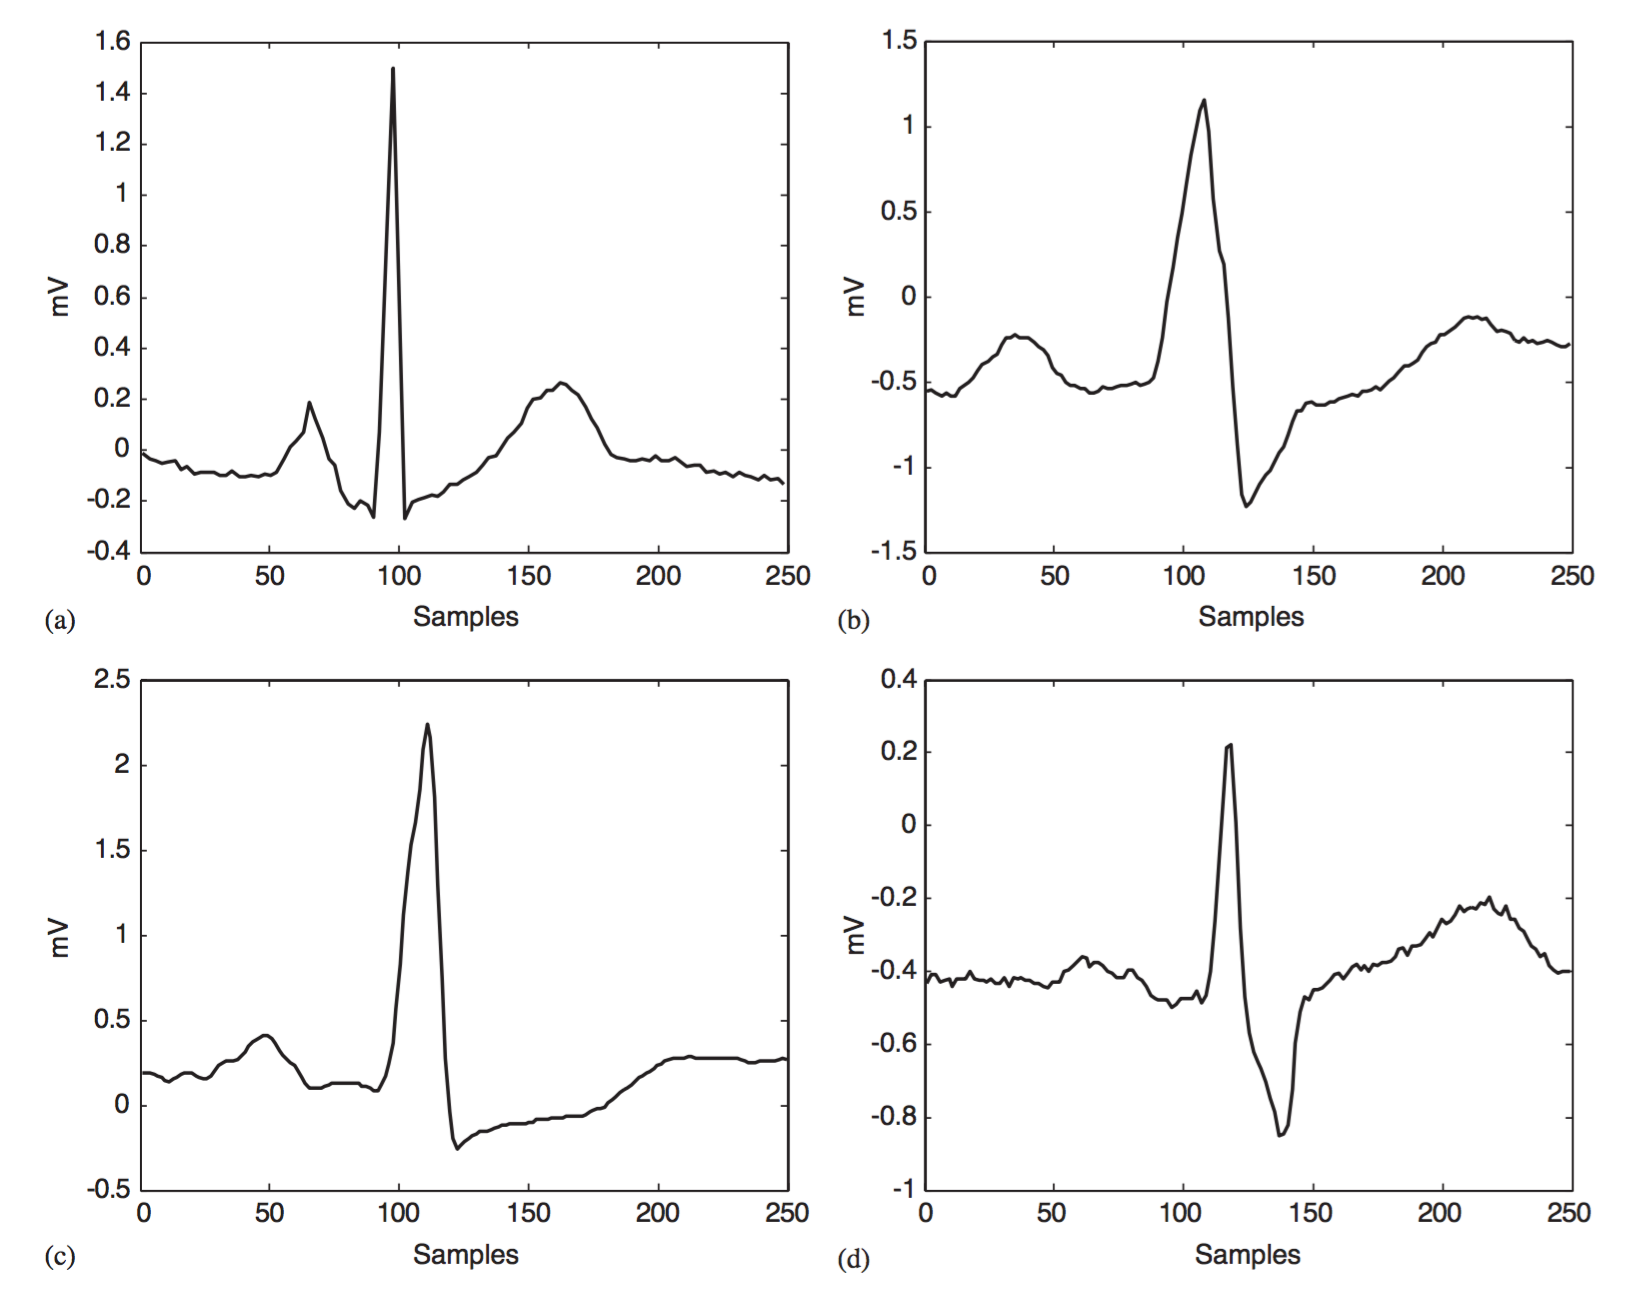
\includegraphics[width=3.5 in]{eps/figure2_ecg_beats.png}
% where an .eps filename suffix will be assumed under latex, 
% and a .pdf suffix will be assumed for pdflatex; or what has been declared
% via \DeclareGraphicsExtensions.
\caption{Waveforms of the ECG beats: (a) Typical N label for normal beat; (b) Typical S label for congestive heart failure beat; (c) Typical V label of Ventricular tachyarryhthmia beat; (d) Typical V label of atrial fibrillation beat.}
\label{figure2}
\end{figure}

\subsection{Electrocardiography Classification Tasks}

\begin{table*}[]
\begin{center}
\begin{threeparttable}
\caption{AAMI Classes Mapped from MIT-BIH Arrhythmia \& Long-term Database Types}
\label{Table1}
\begin{tabular}{cllllll}
\hline
& AAMI heartbeat classes & N & S & V & F & Q \\
& Description  &Any heartbeat not in & Supraventricular ectopic  & Ventricular ectopic  & Fusion beat & Unknown beat \\
&                     &the S,V,F or Q class & beat   		     & beat	      &	     &          \\
\hline
& MIT-BIH heartbeat  &Normal beat (1)            & Aberrated atrial premature & Ventricular escape & Fusion of ventricular& Paced beat (12)\\
&  types (codes)   &  					  &  beat (11)		    &  beat(10)	            & \& normal beat (6)		      &             \\

&                     &Left bundle branch   &  Nodal (junctional) &Premature ventricular& 	 &  Unclassifiable \\
&                     &block beat (2)            & premature beat (7)    &contraction (5)         &	   & beat (13)   \\

&                     & Right bundle branch & Atrial premature & Ventricular flutter &    &  Fusion of paced  \\
&                     & block beat (3) & contraction (8)     & wave (31) & 	   & and normal (38)  \\

&                     & Nodal escape  & Premature or ectopic & 	     &  &                          \\
&                     & beat (11)	  & supraventricular beat(9) &     &   &     \\

&                     & Atrial escape beat (34)   &  	  				      & 				            & 			      &                          \\
\hline
& MITBIH-AR$^a$(100,687) & 89,925$^b$   & 2,774   & 7,171   & 802    & 15        \\
& MITBIH-LT(667,347) & 600,197  &  150  & 64,090  & 	2,906   & 0       \\

\hline
\end{tabular}
\begin{tablenotes}
\item [a] Recording 102, 104, 107, 217 were removed.
\item [b] The counts listed in the table may differ from other literatures \cite{chaza} due to the computation need.
\end{tablenotes}
\end{threeparttable}

\end{center}
     \end{table*}




%The related experiments in this paper were carried out in two public databased available on Physionet, and a collected unlabelled ambulatory electrocardiography database (unlabelled means there were no electrocardiography experts involved in the interpretation). 

%As Table I illustrated the detail of the MIT-BIH Arrhythmia Database and MIT-BIH Long-term Database which mapped to the AAMI heartbeat classes.



\section{Classification With Deep learning Stacked Autoencoder Structures}
Since the SAE based deep structure was capable to extract representations for the raw inputs, it is simpler and more convenient to extract the features for ECG classification instead of discovery or create features by researchers. Thought it should be mentioned that for clinical reasons some features from the researchers might be great of importance, the features were limited in the morphology aspect, which lacks of the ability to use some importance features in the transform-domain features or statistical representations. Another motivation for the deep features was, in the real use of the long-term ECG monitoring, the variances of the data collection devices and the difference among different objects. For example, different Holter manufactories use different collecting chips, or different analog-to-digital sampling rate, or even different digital signal filter parameters. Another factor is the physiological differences of the objects. According to these factors, using the single morphology or time domain features were insufficient, the probability distribution of a certain class is nonexclusive and has variations over multiple directions in the feature space, which makes it impossible to analyze the waveform point by point in the complicated real situation. More robust and invariant features should be extracted and used in the auto-analysis scenes. It is believed that deep architectures can potentially lead to progressively more abstract features at higher layers of feature, and more abstract features are generally invariant to most local changes of the input\cite{bengio2013representation}.

To tackle with these problems, with the stacked autoencoder model the deep invariant features of raw ECG samples can be learned layer by layer. Same as the traditional learning systems, after the feature extracting process, a classifier would be constructed behind the neural network to finish the classification task (Fig. \ref{figure3}). 

\begin{figure}[]
\centering
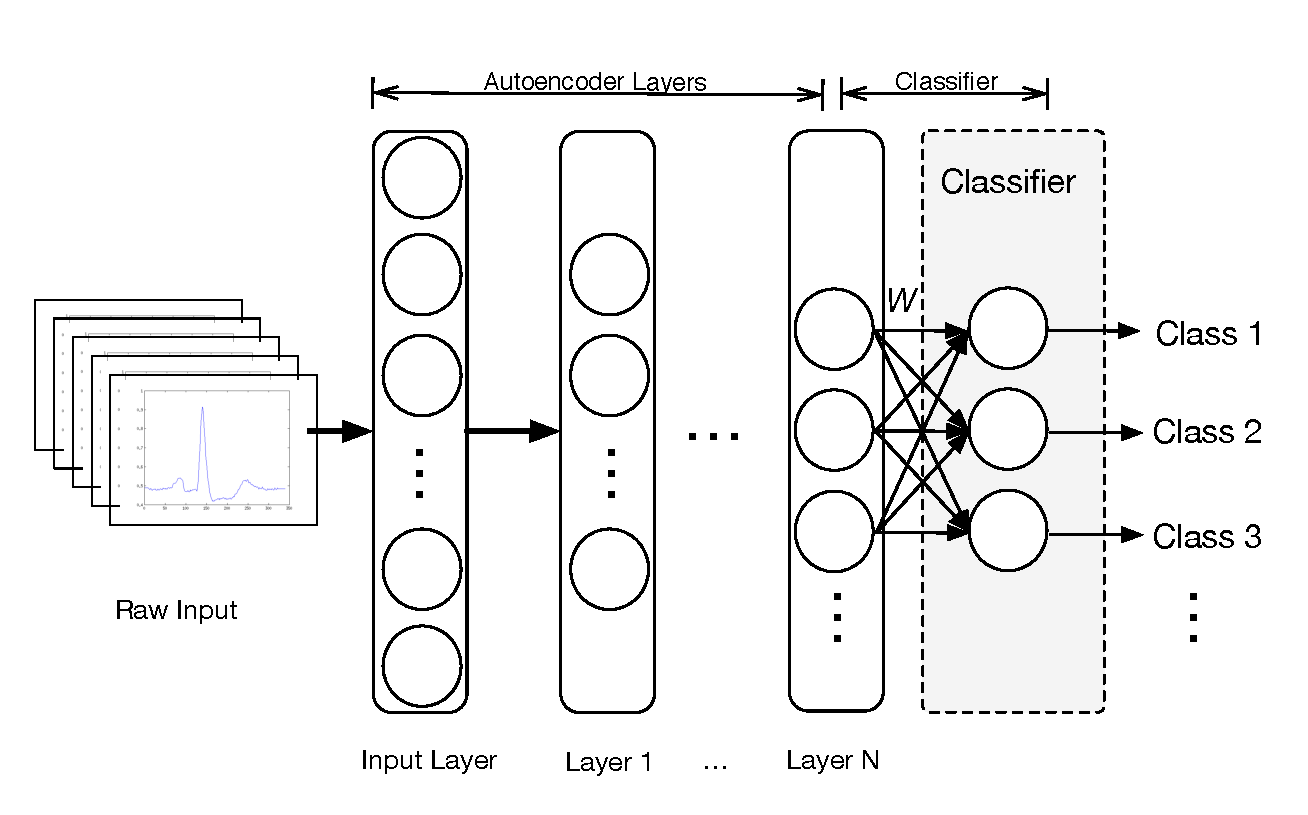
\includegraphics[width=3.5 in]{eps/figure3_classifier.eps}
% where an .eps filename suffix will be assumed under latex, 
% and a .pdf suffix will be assumed for pdflatex; or what has been declared
% via \DeclareGraphicsExtensions.
\caption{The multi-layer autoencoder with a subsequent classifier.}
\label{figure3}
\end{figure}

\subsection{Hierarchal Pre-training}

\subsubsection{Sparsity}
In order to guarantee the representation expression ability of the model, a sparsity constraint is imposed on the hidden units. Let $a_{j}^{(l)}$ denotes the activation (output of the activation function $f(\cdot)$, in the input layer, $a_i^{(1)}=x_i$), then
\begin{equation}
\hat{\rho}_j = \frac{1}{m} \sum_{i=1}^m [{a_j^{(2)}}{(x^{(i)})}]
\end{equation}
denotes the average activation of hidden unit $j$ (averaged over the training set). Approximately enforce the constraint:

\begin{equation}
\hat{\rho}_j = \rho
\end{equation}
where $\rho$ is a sparsity parameter, typically a small value close to zero (such as $\rho = 0.05$), which means the average activation of each hidden neuron $j$ to be close to zero (0.05 for instance). 
To satisfy the constraint of sparsity, an extra penalty term to the optimisation objective that penalised $\hat{\rho}_j $ deviating significantly from $\rho$. The Kullback-Leibler (KL) divergence:

\begin{equation}
 \sum_{j=1}^{s_2}KL(\rho||\hat{\rho}) =  \sum_{j=1}^{s_2}\rho \text{log}{\frac{\rho}{\hat{\rho}_j}}+(1-\rho)\text{log}\frac{1-\rho}{1-\hat{{\rho}_j}}
\end{equation}

\noindent is chosen as the  penalty term. KL-divergence is a standard function for measuring how different two different distributions are. 
\subsubsection{Cost Function}
The first step is to learn a deep feature for the ECG samples via pretraining the SAE hierarchically. In Section II, the outline of training method had been derived. Mathematically, the overall cost function of neural network is denoted by $J(W, b)$ which was defined by:
\begin{equation}
\begin{split}
J(W,b) = [\frac{1}{m}\sum_{i=1}^m(\frac{1}{2}{\|{h_{W,b}(x^{(i)})} - y^{(i)}\|}^2)] \\
+ \frac{\lambda}{2}\sum_{l=1}^{n_l-1} \sum_{i=1}^{s_l} \sum_{j=1}^{s_l+1}{W_{ji}^{(l)}}^2
\end{split}
\end{equation}
in the first part of which is an average sum-of-square error term: $x$ is the input as the training examples; $y$ denotes the output values (in the autoencoder case, $y$ was set as $y=x$); $(x^{(i)}, y^{(i)})$ denotes the $i$-th training example; $W^{(l)}_{(ij)}$ denotes the weights of the connections between unit $j$ in layer $l$, and unit $i$ in layer $l+1$; $b_i^{(l)}$ denotes the bias term associated with unit $i$ in layer $l+1$. For the regularization term which tends to decrease the magnitude of the weights and helps prevent of overfitting: $\lambda$ was adopted as the weight decay parameter while $n_l$ stands for number of layers, $s_l$ denotes number of units in layer $l$.
Add the sparsity parameters, in the autoencoder neural network training, the cost function of $J_{sparse}(W,b)$ was defined as:
\begin{equation}
J_{sparse}(W,b) = J(W,b) + \beta \sum_{j=1}^{s_2}KL(\rho||\hat{\rho_j})
\end{equation}
\noindent $\beta$ denotes the weight of the sparsity penalty term. 


\subsubsection{Activation Function}
The nonlinear mapping activation function $f(\cdot)$ is set to be a $sigmoid$ function:
\begin{equation}
f(x) = \frac{1}{1+e^{-x}}
\end{equation}
both in the ``encoder" and ``decoder". While training the autoencoder, the "tied weights" are used with the greedy layer-wise approach. 

\subsubsection{Training}
The stacked autoencoder consists multiple layers of sparse autoencoders in which the outputs of each layer is wired to the inputs of the successive layer. Sequently we use the definitions above, let $W^{(k)}, \hat{W}^{(k)}, b^{(k)}, \hat{b}^{(k)},$ denote the parameters for the $k$-th autoencoder. The encoding step for the stacked autoencoder is given by running the encoding step of each layer forwardly:
\begin{equation}
a^{(l)} = f(z^{(l)})
\end{equation}
\begin{equation}
z^{(l+1)} = W^{(l)}a^{(l)} + b^{(l)}
\end{equation}
The decoding step is given by running the decoding stack of each autoencoder in reverse order (in the reconstruction encoding and decoding structure):
\begin{equation}
a^{(n + l)} = f(z^{(n + l)}) 
\end{equation}
\begin{equation}
z^{(n + l + 1)} = \hat{W}^{(n - l)}a^{(n + l)} + \hat{b}^{(n - l)}
\end{equation}
After training the network, the reconstruction layers are removed, then stacked autoencoder is constructed with encoders layer by layer. The learned features which we interested in is contained within $a(n)$, which is the activations of the deepest layer of hidden units. 


This vector gives us a representation of the input in terms of higher-order features, which can be used for classification problems by feeding $a(n)$ to a classifier.

\subsection{Fine-Tuning and Classification}
To utilize the learned feature integrate the networks structure, we need to fine-tune the pre-trained network, which uses softmax as the output-layer activation. Softmax ensures the activation of each output unit sums to 1, so that we can deem the output as a set of conditional probabilities. Fine tuning treats all layers of a stacked autoencoder as one single model, so we can improve all the weight parameters in one iteration.



\section{Experimental Results}







\section{Discussion and Conclusions}








\section*{Acknowledgment}
This study was financed partially by the National 863 Program of China (Grant No. 2012AA02A604), the Next generation communication technology Major project of National S\&T (Grant No. 2013ZX03005013), the Key Research Program of the Chinese Academy of Sciences, and the Guangdong Innovation Research Team Funds for Image-Guided Therapy and Low-cost Healthcare. 
% Can use something like this to put references on a page
% by themselves when using endfloat and the captionsoff option.
\ifCLASSOPTIONcaptionsoff
  \newpage
\fi

% trigger a \newpage just before the given reference
% number - used to balance the columns on the last page
% adjust value as needed - may need to be readjusted if
% the document is modified later
%\IEEEtriggeratref{8}
% The "triggered" command can be changed if desired:
%\IEEEtriggercmd{\enlargethispage{-5in}}

% references section

% can use a bibliography generated by BibTeX as a .bbl file
% BibTeX documentation can be easily obtained at:
% http://www.ctan.org/tex-archive/biblio/bibtex/contrib/doc/
% The IEEEtran BibTeX style support page is at:
% http://www.michaelshell.org/tex/ieeetran/bibtex/
%\bibliographystyle{IEEEtran}
% argument is your BibTeX string definitions and bibliography database(s)
%\bibliography{IEEEabrv,../bib/paper}
%
\bibliographystyle{IEEEtran} % Style BST file
\bibliography{bare_jrnl}  
% <OR> manually copy in the resultant .bbl file
% set second argument of \begin to the number of references
% (used to reserve space for the reference number labels box)
%\begin{thebibliography}{2}

%\bibitem{tanis}
%T.~Mar, S.~Zaunseder, J.P.~Martinez, M.~Llamedo and R.~Poll, \emph{Optimization of electrocardiography Classification by Means of Feature Selection}.\hskip 1em plus
%  0.5em minus 0.4em\relax Harlow, England: Addison-Wesley, 1999.
  
%\bibitem{care}
%H.~Kopka and P.~W. Daly, \emph{A Guide to \LaTeX}, 3rd~ed.\hskip 1em plus
%  0.5em minus 0.4em\relax Harlow, England: Addison-Wesley, 1999.
  
%\end{thebibliography}

% biography section
% 
% If you have an EPS/PDF photo (graphicx package needed) extra braces are
% needed around the contents of the optional argument to biography to prevent
% the LaTeX parser from getting confused when it sees the complicated
% \includegraphics command within an optional argument. (You could create
% your own custom macro containing the \includegraphics command to make things
% simpler here.)
%\begin{IEEEbiography}[{\includegraphics[width=1in,height=1.25in,clip,keepaspectratio]{mshell}}]{Michael Shell}
% or if you just want to reserve a space for a photo:

\begin{IEEEbiography}{Jan Doe}
Biography text here.
\end{IEEEbiography}
% if you will not have a photo at all:
\begin{IEEEbiographynophoto}{John Doe}
Biography text here.
\end{IEEEbiographynophoto}

% insert where needed to balance the two columns on the last page with
% biographies
%\newpage

\begin{IEEEbiographynophoto}{Jane Doe}
Biography text here.
\end{IEEEbiographynophoto}

% You can push biographies down or up by placing
% a \vfill before or after them. The appropriate
% use of \vfill depends on what kind of text is
% on the last page and whether or not the columns
% are being equalized.

%\vfill

% Can be used to pull up biographies so that the bottom of the last one
% is flush with the other column.
%\enlargethispage{-5in}

% that's all folks
\end{document}


